\title{Computer Architecture - CS 301} % You may change the title if you want.

\author{Rishit Saiya - 180010027, Assignment - 9}

\date{\today}

\documentclass[12pt]{article}
\usepackage{fullpage}
\usepackage{enumitem}
\usepackage{amsmath,mathtools}
\usepackage{amssymb}
\usepackage[super]{nth}
\usepackage{textcomp}
\usepackage{hyperref}
\begin{document}
\maketitle

%----------------------------------------------------------------
\section{}
Given that our address size is \textbf{32-bit}. Additionally we are given that line size is \textbf{64B} and cache is of size \textbf{1kB}. In this problem, we are supposed to illustrate our approach on how cache will search the address A (32-bit) for 3 various cases namely: Direct Mapped Cache, Fully Associative Cache \& 2-way set Associative Cache.

The Number of Entries (N) will be calculated as follows:
\begin{equation*}
    N = \frac{CS}{LS}
\end{equation*}
where CS is the cache size and LS is the Line Size. \\

In this case, it would be as follows:
\begin{equation*}
    N = \frac{2^{10}}{2^6}
\end{equation*}
or,
\begin{equation*}
    N = 2^4
\end{equation*}
or,
\begin{equation*}
    N = 16
\end{equation*}
We know that definitions of Data array and Tag Array which are contents of block \& a entity of the block address such that the block can be uniquely identified respectively. [Source - Video Lecture].
%----------------------------------------------------------------
\subsection{Direct Mapped Cache}
Before we try to illustrate on approach of Direct Mapped Cache, let's understand about Direct Mapped Cache. \\

In this technique, we map each block of main memory into only one possible cache line. In other words, we assign each memory block to a specific line in the cache.
\begin{verbatim}
  if(Line is taken up prior by a memory block, when loading is done){
      Trash (Old Block);
  }  
\end{verbatim}
As main literature suggests, an address space is split into two parts index field \& a tag field. The cache is used to store the tag field whereas the rest is stored in the main memory. However the problem here is that each block can be mapped only to 1 entry only. \\

\begin{table}[]
\begin{center}

\begin{tabular}{|l|c|l|}
\hline
\textbf{Tag (22 bits)} & \textbf{Index (4 bits)} & \textbf{Offset (6 bits)} \\ \hline
\end{tabular}
\caption{Address format for Direct Mapped Cache}
\end{center}
\end{table}
As mentioned in Table 1, Address format is mentioned. We know that in Direct Mapped method, the index is calculated in the following way:
\begin{equation*}
    Index = BA(A) \,  modulo \, N
\end{equation*}
where BA(A) is the Block Address of A and N (16 in this case) is the number of entries. \\

The tag comparison essentially is 22 MSB bits of the address A.
So by that logic, the last 4 bits of the address after removing offset (6 bits), we then access entry, index in the tag array of address and then compare the contents of the tag. 
Later we follow the logic:
\begin{verbatim}
     If (match = Hit){
         Hit;
     }
     else{
         Miss;
     }
\end{verbatim}
In this way, the contents are read from the data array of the matching entry. 
%----------------------------------------------------------------
\subsection{Fully Associative Cache}
Before we try to illustrate on approach of Direct Mapped Cache, let's understand about Fully Associative Cache. \\

In this technique, the associative memory is used to store content and addresses of the memory word. It means that any block can go into any line of the cache. We use the word id bits to identify which word in the block is needed, but the tag becomes all of the remaining bits in address. This enables the placement of any word at any place in the cache memory.  \\

Some issues which were mentioned in the video were that the tag array consists CAM arrays and they are larger and slower. This is not very power efficient because we need to compare the block address with every single entry on the tag array as mentioned above. Some patches for power issues are mentioned in Razor DVS Technique (seminar topic). \\

\begin{figure}
    \centering
    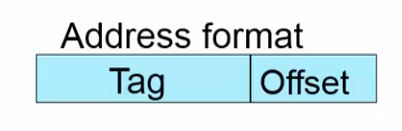
\includegraphics{Assignment-9/fully_associative_cache.png}
    \caption{Fully Associative Cache}
\end{figure}

Figure 1 shows address format of Fully Associative Cache. Here, according to the concept, we see that Tag has \textbf{26 bits} and Offset is \textbf{6 bits}. 

As mentioned in the video, an array of CAM cells is used for the 22 bit long tag array. We follow the below logic (the tag comparison is essentially with 26 MSB of address):
\begin{verbatim}
    Compare entry with Tag;
    Match Line = 1;
\end{verbatim}
It means that each entry would compare its contents with the tag in the above mentioned fashion and the match line is set to 1. Later, the OR gate computes a hit or miss. The encoder mentioned in the lecture then computes the index of the matched entry and in this way, the contents are read from the data array of the matching entry. However we have to note that index will be 4 bits long here because there are 16 entries.
%----------------------------------------------------------------
\subsection{2-way Set Associative Cache}
Before we try to illustrate on approach of Direct Mapped Cache, let's understand about k-way set Associative Cache. \\

In this technique, the set associative addresses the problem of possible thrashing in the direct mapping method. We do this by saying that instead of having exactly one line that a block can map to in the cache, we will group a few lines together creating a set. Then a block in memory can map to any one of the lines of a specific set. So, in the Set-associative mapping, it allows that each word that is present in the cache can have two or more words in the main memory for the same index address. \\ 

\begin{table}[]
\begin{center}
\begin{tabular}{|l|c|l|}
\hline
\textbf{Tag (23 bits)} & \textbf{Index (3 bits)} & \textbf{Offset (6 bits)} \\ \hline
\end{tabular}
\caption{2-way Set Associative Cache Address Format}
\end{center}
\end{table}

For a k-way association, we divide tag array in sets of k entries. Table 2 shows the address format for the 2-way Set Associative Cache.\\

In this case it is 2. So, we now have a 23 bit long tag array and 3 bit long index in the address. With the same idea as above, we access indices and then read all the tags in the given set. We then compare the tags with the address tag. Later, OR gate is used to compute a hit/miss as above. Then encoder as mentioned in lecture finds the index of the matched entry. It is to be noted that we have 8 indices (obtained by 16/2) where each index pointing to a set of 2 entries in the address.

\section{Conclusion}
This part is written by help of video lecture.

When we try to compare the \textbf{\textit{Speed of Caches}}, we see that Direct Mapped Cache performs the best. It is then followed by k-Set Associative Cache and finally follows Fully Associative Cache. \\

When we try to compare the \textbf{\textit{Hit Rate of Caches}}, we see that Fully Associative Cache performs the best. It is then followed by k-Set Associative Cache and finally follows Direct Mapped Cache. \\

As also given in the lecture, there is this small trade off for choosing the best method of Cache. But as we can see, it is better to safe by choosing K-set Associative Cache as it provides optimum speed and hit rate.
%----------------------------------------------------------------
\end{document}